%Templated from IEEE Preparation Papers
\documentclass[letterpaper, 10 pt, conference]{ieeeconf}

\IEEEoverridecommandlockouts                              % This command is only
                                                          % needed if you want to
                                                          % use the \thanks command
\overrideIEEEmargins
% See the \addtolength command later in the file to balance the column lengths
% on the last page of the document



%The following packages can be found on http:\\www.ctan.org
\usepackage{graphics} % for pdf, bitmapped graphics files
\usepackage{epsfig} % for postscript graphics files
\usepackage{mathptmx} % assumes new font selection scheme installed
\usepackage{times} % assumes new font selection scheme installed
\usepackage{amsmath} % assumes amsmath package installed
\usepackage{amssymb}  % assumes amsmath package installed
\usepackage{float}


\usepackage{url}


\title{Database Storage}

\author{ \parbox{3 in}{\centering Will Wu\\
        Electrical and Computer Engineering\\
        University of Rochester\\
        500 Computer Studies Building \\
        Rochester, NY 14627\\
        {\tt\small ywu37@ur.rochester.edu}}
}



\begin{document}


\maketitle
\thispagestyle{empty}
\pagestyle{empty}


%%%%%%%%%%%%%%%%%%%%%%%%%%%%%%%%%%%%%%%%%%%%%%%%%%%%%%%%%%%%%%%%%%%%%%%%%%%%%%%%
\begin{abstract}
The amount of data generated on the internet grows at approximately 40 percent every year. \cite{13}  With an ocean of data to wade through, an organization structure is paramount to make the data understandable to the bounded human mind.  Databases are a great tool for organizing relationships among objects in the data.  Its scalability and utility outshines spreadsheets such as the ones made in Excel.  New relations in the form of tables can be made very easily and can be linked to existing relationships.  Modifications of relationships require much less effort on the behalf of the user.  However, modifications are made with the utmost scrutiny as functional dependencies are checked.  This prevents accidental human error from breaking relationships or losing data altogether. 

Databases have been incorporated into most large systems and due to its scalability, it is not uncommon to see databases with thousands of entries of object data.  The largest of current databases reach magnitudes of petabytes $(1000^5)$.  How such a large magnitude of data can be stored and maintained on hardware is an interesting question to contemplate.

Storing digital data has an extensive hierarchy of different technologies.  The entire hierarchy can be broken down into three sections, with each level farther away from the processing unit and capable of holding more data.  They are unexcitingly named the primary storage hierarchy, the secondary storage hierarchy, and the tertiary storage hierarchy.  This paper will focus on primary and secondary storage devices.  

This paper introduces and discusses on important topics in memory storage with an emphasis on how hardware and data structures assist in storing large databases, accessing and modifying database object data stored within, and accommodating multiple users. 

\end{abstract}


%%%%%%%%%%%%%%%%%%%%%%%%%%%%%%%%%%%%%%%%%%%%%%%%%%%%%%%%%%%%%%%%%%%%%%%%%%%%%%%%



\section{TERMINOLOGY}
When discussing memory systems, a distinction is made between the data being read and manipulated by end users and the data that describes the object data, also known as metadata.  To cement this distinction, suppose a database contains an integer age entry of the value “50”.  The size needed to store this entry is 32 bit (the size of an integer).  We refer to the entry of “50” as object data and the “32” which references the size needed to store the object data “50” as metadata.

The terms hot and cold are used to describe devices and object data.  For instance, a cache is considered cold when it contains data not to be accessed by the processing unit in the near-past and near-future.  Similarly, object data is hot when it is currently accessed often and cold if it has not been accessed in a significant amount of time. [5]

Granularity is a term that refers to the minimum size that data that can be divided into.  Pages are typically transferred between the backing store secondary storage and DRAM.  A finer granularity example is the block-based memory transfers between DRAM and SRAM.  Typically, as data granularity increases or becomes more fine, methods of optimizations can be more easily developed, however this comes at the expensive of more storage or processing overhead.

Operating systems provide processes a level of abstraction between the physical RAM and the amount of RAM a process can operate with.  Virtualization of memory allows for more freedom in the storage and usage of memory for both the process and the operating system.  The matter of fact is that there are significantly more virtual pages wanting to be accessed than there are physical pages that the main memory can accommodate.  Virtual to physical address translation provides every individual process running at the same time on an operating system an illusion of memory exclusivity.  This allows the main memory to accommodate multiple different processes.  This allows the operating system to switch execution of one process to another process more easily.  The operating system provides a table that translates virtual page addresses to physical page addresses.

\begin{figure}[H]%Figure 1: Virtual address Physical address translation
	\centering
	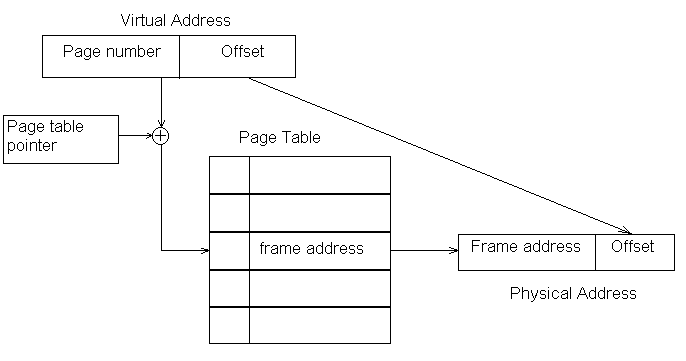
\includegraphics [width=0.5\textwidth] {Figures/Virtual Physical Address Translation.png} 
    \caption{Virtual Physical Address Translation}
\end{figure}


Modern-day digital storage devices dedicate extra bits to metadata in order to implement data error detection and data error correction.  Hamming distance is the number of differing bits between two bit strings.  This value is used along with the cyclic redundancy check to correct small bit corruptions.
\newpage

\section{THE NATURE OF DATABASES}
Databases have become an extremely efficient method of storing large amounts of data and maintaining complex relationships between specific pieces of data.  This pales in comparison to some spreadsheet applications which only provide a grid structure to input data and do very little to assist with connections among pieces of data.

Databases have matured over the years to contain many features.  The database management system (DBMS) is a piece of software system that facilitates manipulation and access to data in the database.  Nearly all object data is stored in the form of variable-length character arrays when translated to the hardware domain.

\section{THE NATURE OF THE STORAGE HIERARCHY}

\subsection{Random Access Memory}
The primary storage hierarchy encompasses the static and dynamic random access memory devices.  They devices noticeably reside within the confines of the same computer as the processing unit it serves.  SRAM typically make up of CPU caches which reside on the same chip as the processing unit.  Sticks of DRAM are attached to the motherboard and function as the “main memory”.  For some small to medium sized databases, it is quite reasonable to fit the entire database in DRAM chips.  Primary storage devices are considered volatile.  This term is defined as storage that requires a consistent power source in order to maintain state.  For instance, if the computer is powered off, both RAM devices will lose whatever data was stored on them.

\subsection{Hard Disk Drive}
Hard disk drives (HDD) have been the primary form of large and long term nonvolatile memory storage for computer systems for nearly 50 years.  The term nonvolatile refers to the ability to store information through on and off power cycles.  These devices are comprised of a set of rotating magnetic disks with a motor controlled arm and actuator heads for each disk (See figure 2).  The head at the end of the arm consists of a coil wrapped around a semi-toroid conductor (shape akin to a horseshoe).  This makes the head function as an inductor which allows the head to induce the ferromagnets on the surface of the disk to align to a certain orientation based on the direction of the magnetic field induced from the current through the coil.  Data is stored on the surface of the disk by inducing the electromagnet residing in each compartment.  Reading involves the head of the arm detecting the changes in magnetic field along the surface of the disk. \cite{5}

\begin{figure}[H] %Figure 2: Anatomy of disk drive with arm and rotating spindles [15]
	\centering
	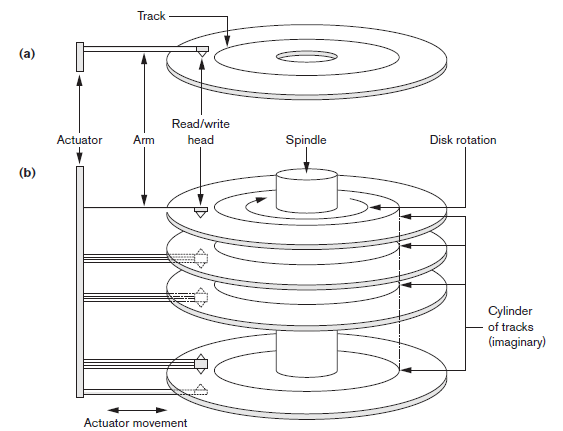
\includegraphics [width=0.5\textwidth] {Figures/Anatomy of Disk Drive.png} 
    \caption{Anatomy of disk drive with arm and rotating spindles \cite{15}}
\end{figure}

% 
\begin{figure}[H] %Figure 3: The anatomy of a hard disk drive sector. [5]
	\centering
	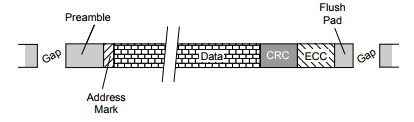
\includegraphics [width=0.5\textwidth] {Figures/HDD Sector.png} 
    \caption{The anatomy of a hard disk drive sector. \cite{5}}
\end{figure}


\begin{figure}[H] %Figure 4: The process of writing to disk. [5]
	\centering
	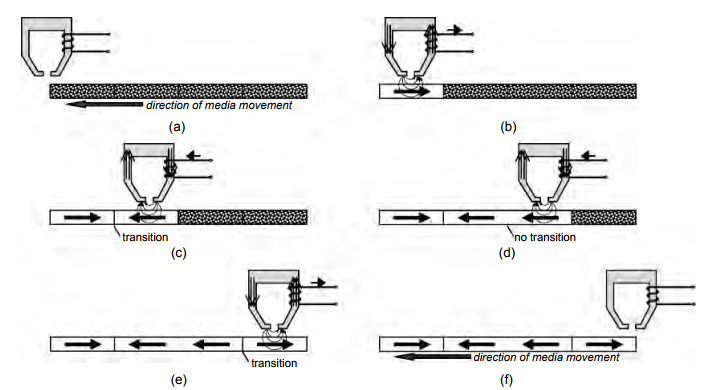
\includegraphics [width=0.5\textwidth] {Figures/Writing to Disk.png} 
    \caption{The process of writing to disk. \cite{5}}
\end{figure}

\begin{figure}[!h] %Figure 5: Anatomy of NAND flash memory [10]
	\centering
	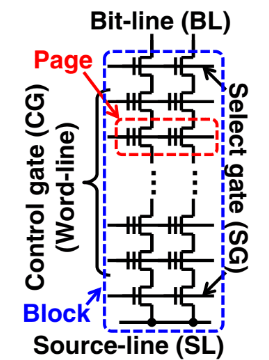
\includegraphics [width=0.5\textwidth] {Figures/NAND Flash Memory.png} 
    \caption{Anatomy of NAND flash memory \cite{10}}
\end{figure}  

\subsection{Flash Memory}
Flash memory is the newest device to the industry and is implemented in familiar consumer electronics in the form of Flash drives (colloquially also referred to as thumb-stick drives) and Solid-State Drives (SSD).  SSDs provide an alternative to HDDs boasting no spinning disk platters.  This translates to lower latencies as it is not limited by the mechanical limitations of the rotating motor found in HDDs. [6]  Flash memory comprises of NAND and NOR logic gates connected in series in an array of word lines and bit lines. [10]




Flash memory has also virtual/physical address translation data structures referred to as the Flash Translation Layer (FTL).  This is done to handle repeated writes to the same logical address and to figure out which large blocks to erase.
Perform wear-leveling to extend the NAND flash chip’s lifetime, and to execute garbage collection to reclaim free memory [10]
Se has row size of 100 bytes which is much smaller than the NAND memory page size of 16KB.  This puts more pressure on data fragmentation and the need for garbage collection.

%Minimum write data unit for SSD is a page.  Pages are set valid or invalid. Physical overwrite is not allowed.
\section{Overview of HDD RAID Levels}
Back in 1988, David Patterson, Garth Gibson, and Randy Katz proposed a standard magnetic disk storage standard.  In an incredibly avant-garde paper, they proposed a system of Redundant Array of Independent Disks (RAID) as a method of improving “performance, reliability, power consumption, and scalability” over the convention of the time: Single Large Expensive Disk (SLED) [3].  Hard disk drives today are developed in accordance with the RAID standard.  RAID 0 was its first incarnation and provided only byte-level striping across multiple disks.  Notably, RAID 0 provides neither data redundancy nor parity information.  Simply, object data is stored only once and with no accompanying metadata.  This configuration is incredibly fragile as it is not tolerant to errors of any sort.  If data is corrupted, there is no method of correcting it and the end user is likely to encounter bogus results.  Byte-level striping requires the arm in each disk array to read the same index simultaneously.  This can be implemented by the disk rotary motor and arm motor being in lockstep synchronization.  RAID 1 introduces redundancy in its first form: mirroring.  In RAID 1, the object is stored twice on separate disk arrays.  One functions as a spare in the event that the primary disk no longer functions or develops data corruption.  Error correction is not a supported in the RAID 1 configuration.  One feature of this configuration is its emphasis on memory reads over memory writes.  Memory writes are very costly as the data much be written to each functional disk array in the configuration.  Memory reads can be satisfied by reading only one operational disk array.  RAID 2 introduces error correction in the form of Hamming distance correction code.  

RAID 3 iterates the metadata configuration to a disk dedicated to metadata.  The Hamming distance code is accompanied with parity check codes.  Notice one weakness of this configuration is the heavy importance put on the parity check disk.  The parity check disk is written to for every memory write.  It is not hard to imagine that this uneven load likely causes the parity check disk to deteriorate more quickly than any other disks housing object data.  Even worse, if the disk containing the parity check completely fails, then the disk configuration functionally is equivalent to the RAID 0 configuration.  This weakness was swiftly corrected with the introduction of RAID 5 later.  RAID 4 changes the paradigm from byte-level striping to block-level striping.  The change from byte-level striping to block-level striping allows for multiple random reads to be accommodated.  The heads of the disk arrays no longer have to maintain lockstep synchronization to satisfy memory reads.

RAID 5 decides to reorganize how object data and metadata is stored.  The error detection and correction metadata is not distributed among all of the disks.  RAID 5 is the standard for modern HDD storage.

Each of the RAID configurations provide some slightly different features.  RAID configurations can be combined to make nested or hybrid RAID configurations.  These combinations have multi-digit designations.  The denomination guideline is as follows:

\begin{itemize}
    \item The left-most digit represents the RAID level of neighboring disks.
    \item Each disk groupings is abstracted as one disk array for the purposes of the next level of RAID.
    \item The next digit represents the RAID level of the disk arrays.
\end{itemize}

The standard for modern day database storage is some combinations of RAID levels 0, 1, and 5 with most proprietary database systems operating with RAID 10.


\begin{figure}[H] %Figure 6: Nested RAID 10 \cite{14}
	\centering
	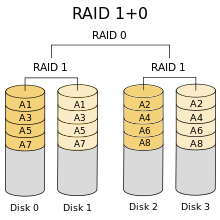
\includegraphics [width=0.5\textwidth] {Figures/Nested RAID 10.png} 
    \caption{Figure 6: Nested RAID 10 \cite{14}}
\end{figure}


\section{THE COST OF LARGE OBJECTS}
Now that we have established that disks are physical pieces of electromagnets, it is conceivable how such a device can fail.  Disk failure is a point where the data on the disk is corrupted in such a way that the ECC and CRC mechanisms can no longer recover the object data.  Disk manufacturers calculate the Mean Time to Failure (MTTF) which expectedly is the lifetime a memory system is expected to last until its reliability can no longer be guaranteed.  Patterson provides the simple formula for computing the MTTF of a disk array. [3]

\begin{equation}
MTTF_{disk array} = \frac{MTTF_{single disk}}{Number\ of\ Disks\ in\ the\ array}
\end{equation}

One relationship to note is the larger one’s database is, the more disks will be required to store all of that data.  This increases the number of disks in the array, which decreases the MTTF of a disk array.  So the larger a database is, the more likely it is to fail!  Storing that same database in a RAID memory system with redundancy provides spare disks in the event of data corruption or hardware failure.
 


\begin{equation}
%\begin{aligned}
$$MTTF_{RAID\ group}$$ = \frac{MTTF_{disk}}{Disks\ in\ the\ group + Number\ of\ Spares} 
* \frac{1}{P(Failure\ Before\ Repair)}
%\end{aligned}
\end{equation}

\begin{equation}
$$P(Failure\ Before\ Repair)$$ = \frac{MTTR}{MTTF_{Disk} / (Disks\ in\ the\ group + Number\ of\ Spares - 1)}
\end{equation}

Lock Gross (LG) is defined as product of all data objects multiplied by the transaction execution time.  This metric means not very much by itself but is used to evaluate transaction concurrency.
 
\begin{equation}
LG = Execution\ Time\ of\ Transaction * \sum_{i=1}^{n}{Number\ of\ Objects_i}
\end{equation}
 
Concurrence degree (CD) of a transaction is the sum of LG when performed independently divided by the sum of LGs when transactions are done sequentially.

\begin{equation}
CD = \frac{\sum_{i=1}^{k}LG_i}{LG}
\end{equation}

The concurrence degree metric provides an interesting optimization when executing database transactions.  The concurrence degree is always a number between the values 0 and 1.  The sequential lock gross should always be larger than the independent sum of lock gross values.  This is because the transition time between database transaction is nonzero.  Deadlock decreases the concurrence degree.  The smaller the lock granularity, the greater the concurrence degree. [3]

\section{DATABASE MEMORY ACCESS PATTERNS}
It is no secret that processing units of today are lightning fast.  Clock speeds for consumer CPUs commonly boast gigahertz of clock speed in addition to many optimization features such as multiple cores, ever smaller transistor sizes, faster PCI-express bus speeds and wider bus widths, and graphical capabilities.  Meanwhile, memory systems have made innovations at a much slower pace and with much less fanfare.  This disparity between the speeds of the processing units and memory units is colloquially referred to as the “memory wall” or “bandwidth wall” [9].  Looking at modern day workload recipes, still a large section of time is spent on data accesses to the secondary storage system. In order to make the most impactful progress towards reducing execution time, emphasis must be put on reducing the execution time of memory accesses as opposed to the execution time of processing.  This phenomenon is described in Amdahl’s Law.  In order to reduce time spent with memory access, a thorough analysis of the pattern of memory accessed should be made.  Doing so will give some intuitions on how optimizations can be made.

Stonebraker’s paper succinctly categorized database accesses into four bins:

\begin{enumerate}
    \item Sequential access to blocks which will not be referenced.
    \item Sequential access to blocks which will be cyclically referenced.
    \item Random access to blocks which will not be referenced again.
    \item Random access to blocks for which there is a nonzero probability of reference.
\end{enumerate}

Human intuition has a strong preference towards least recently used eviction protocol should be used as it used for general computing.  LRU is perfect for workloads of type 4 as it most accurately describes general computing.  As counterintuitive as it seems, most recently used eviction protocol should be used for workloads of type 1 and 3 [1].  This interestingly enough slightly increases the page miss rate over the long term.  Modern DBMS are able to identify the memory access patterns.

\section{DATABASE OPERATIONS}
Database transactions are processed using transaction managers and resource locks.  ZhangBing Li’s paper coins this process as the two-phase locking protocol.  Each transaction manager (TM) contains a lock manager (LM) and data processing unit (DP).  The global dictionary(GD) provides a resource that dictates which global locks will be needed for any transaction.  

The lock data structure is utilized during database transactions in order to maintain integrity and concurrency when manipulating both object data and metadata when multiple requests are made on the same object data.  There exists a lock hierarchy utilized when handling database transactions.  This lock hierarchy include shared, update, and exclusive locks.  When transactions can be made parallelizable among multiple processing units, distinctions are made between lower priority global locks and higher priority local locks.  One optimization made in lock management is the feature that locks can be changed between lock allocation and lock acquisition.  Locks can be upgraded from one of higher priority to one of lower priority.  

\begin{figure*}[h] %Figure 7: Lock Table and Transaciton Lock List Data Structure [8]
	\centering
	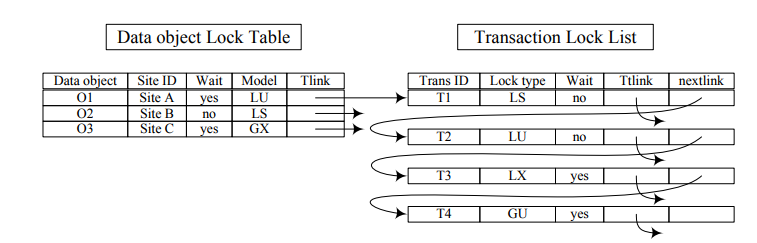
\includegraphics [width=\textwidth] {Figures/Lock Table Transaction Lock List.png} 
    \caption{Lock Table and Transaction Lock List Data Structure \cite{8}}
\end{figure*}

The two-phase locking protocol is as follows:
\begin{enumerate}
    \item The origin or source transaction manager requests for locks.
    \item If all the locks are held in the origin lock manager, the DP will be given a signal to start processing.
    \item If the transaction is a global transaction, the origin TM sends the global locks to the other transaction managers involved.
    \item Each non-origin transaction manager sends all of its locks to its respective lock manager.
    \item The locks in the non-origin lock managers are held and the respective data processing units are given the signal to start processing.
    \item The DP notices the end of the message of its transaction manager and transfers its results to the DP of the origin site.
    \item The DP in the origin site sends a final signal to the original transaction manager that the data has been processed.
    \item The DPs send messages to the originating transaction manager which then decides whether the transaction is submitted or aborted.
    \item When the global transaction is submitted or aborted, the transaction manager in the original site releases all the locks.
\end{enumerate}


\begin{figure}[H] %Figure 8: Two-Phase Locking Protocol [8]
	\centering
	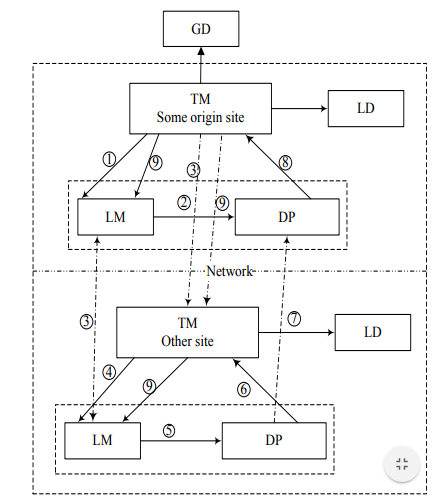
\includegraphics [width=0.5\textwidth] {Figures/Two Stage Lock.png} 
    \caption{Two-Phase Locking Protocol \cite{8}}
\end{figure}
 

Data insertions do not require the acquisition of locks.  Data insertions involve the DP looking for locks that are marked as shared and avoids those spaces.  Valid bid is turned on and new object data is overwritten on top of old invalid data.  Deletions are simply changing the valid bit from 1 to 0.  The object data is not cleared to null data.

\section{DATA ORGANIZATION AND FRAGMENTATION}
One of the most useful features of the database is the ability for users to make new relationships among database entries and add, modify, and remove database entries at will.  One of the simplest forms of data storage is called a heap file.  In a heap file, object data is stored in consecutive virtual addresses in the order they are added to the database or modified.  The tradeoff for the convenience of object data insertion, alteration, and deletion comes at the expensive of searching through that object data.  The object data is unsorted by any object data metric other than the date and time modified.  Curiously enough, if time-order is the only metric of interest.  This heap file organization structure may be desirable for databases focusing on timelines or documentation of events.

As more object data modifications are committed, data becomes suboptimally located.  Data additions in heap files are easy enough commit but typically results in null data at the end of physical pages.  Data deletions result in blocks of invalid data of varying sizes within a physical page.  The worst aspect of this is there are difficulties in filling in the blocks of invalid data with new valid data.  The ratio of object data in a span of a page to the capacity of that page will decrease over time.  This phenomenon is described as data fragmentation.  The DBMS maintains the virtual address space and periodically attempts to move object data such that gaps are consolidated and may be filled up with other object data in a process called defragmentation.  


\section{OPERATING SYSTEM ASSISTANCE}
With the discussion of locks earlier in the paper, the similarities between the locking mechanism and the resource sharing data structures provided by the operating system is uncanny.  One such idea is explored in Michael Stonebraker’s paper.  He discusses how database management operations can be supported by the operating system to improve performance.  Operating systems are of the most help to database operations in the areas of multi-user support and process management.[1]

Blasgen noticed that DBMS processes behave just like any other process and have critical sections.  The entry and exit of these critical sections traditionally require the use of resource locks.  

\begin{figure}[H] %DBMS
	\centering
	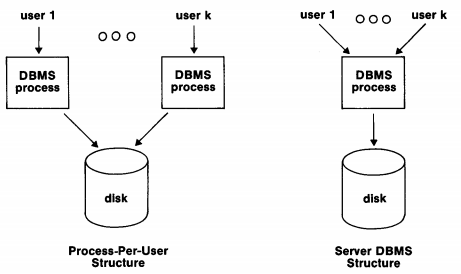
\includegraphics [width=0.5\textwidth] {Figures/DBMS Process Multiple Users.png} 
    \caption{DBMS process structure when accommodating multiple users \cite{10}}
\end{figure}

The process per user structure provides this familiar structure to the operating system.  Operating systems have little issue supporting multiple processes simultaneously.  However, context switching is not desirable for the DBMS as the quantity of user-space data for each user’s DBMS process is very large which significantly increases the cost of context switching.  Allocating each end user its own DBMS process also runs into another issue: concurrency and race conditions among processes when making changes to the database.  A more minimal operating system kernel, called an exokernel, may be more appropriate for DBMS operations.
\newpage
\begin{figure*}[H]%DB Operation
	\centering
	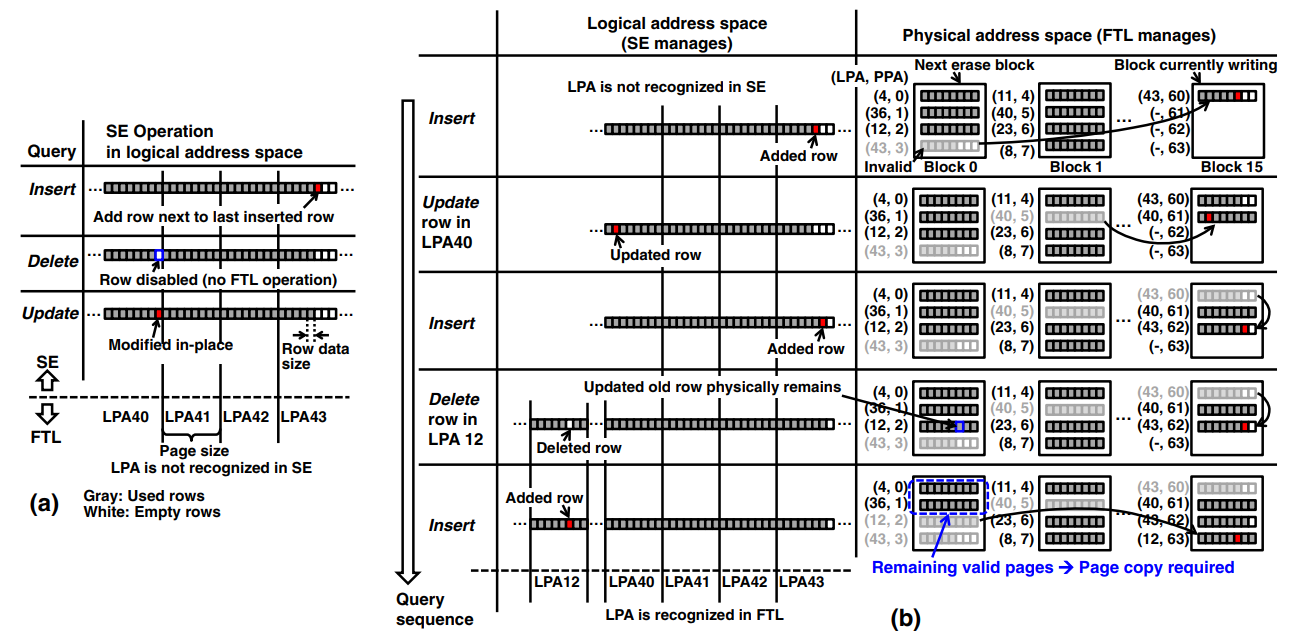
\includegraphics [width=\textwidth]{Figures/DB Operation.png} 
    \caption{Database operation in virtual and physical memory domains \cite{11}}
\end{figure*}
\section{FINAL REMARKS}
The semiconductors industry moves at a blisteringly fast pace courtesy of the fateful extrapolation of four data points from Gordon Moore's paper.  Moore’s Law from that paper hints that the number of transistors on integrated circuits will double approximately every two years.  Just a decade ago, Hitachi introduced the first consumer hard disk drive with a capacity of one terabyte $(1000^4)$.  In 2017, Western Digital released a Helium-based hard disk drive with a space capacity of 12TB.  It would appear that the industry has obliged to maintain the course predicted by Moore.  As a result, technologies become outclassed very quickly.  This presents an interesting economic decision: Who wants to trust 20-year-old hardware to maintain data integrity when the newest hardware can do a much better job?


%\addtolength{\textheight}{-12cm}   % This command serves to balance the column lengths
                                  % on the last page of the document manually. It shortens
                                  % the textheight of the last page by a suitable amount.
                                  % This command does not take effect until the next page
                                  % so it should come on the page before the last. Make
                                  % sure that you do not shorten the textheight too much.


\begin{thebibliography}{99}
\bibitem{1} M. Stonebreaker. 1981. “Operating system support for database management.” Commun. ACM, 24(7), 412–418, July 1981.

\bibitem{2} Omiecinski 1985: E. Omiecinski, Incremental File Reorganization Schemes, Proc. Int’l. Conf. on Very Large Data Bases, Stockholm, Sweden, August 1985, 346. 

\bibitem{3} Patterson, Gibson, and Katz 1988: D. A. Patterson, G. Gibson, and R. H. Katz, A Case for Redundant Arrays of Inexpensive Disks (RAID), Proc. ACM SIGMOD Conf., Chicago, IL, June 1988, 109

\bibitem{4} S. Ng. 1994c. “Sparing for redundant disk arrays.” Distributed Parallel Databases, 2(2), 133–149, 1994.

\bibitem{5} Bruce Jacob , Spencer Ng , David Wang, Memory Systems: Cache, DRAM, Disk, Morgan Kaufmann Publishers Inc., San Francisco, CA, 2007

\bibitem{6} Kemper, A., Neumann, T.: Hyper: A hybrid oltp and olap main memory database system based on virtual memory snapshots. In: ICDE (2011)

\bibitem{7} Gottstein, R., Petrov, I., Buchmann, A.: Aspects of append-based database storage management on flash memories. In: Proc. of DBKDA 2013, pp. 116–120. IARIA (2013) 

\bibitem{8} Zhangbing Li, Zilan Zhu and Shaobo Zhang, ―Locking Mechanism for Distributed Database Systems‖, Journal of Networks, Vol. 9, No. 8, 2014.

\bibitem{9} W.A. Wulf and S.A. McKee, “Hitting the Memory Wall: Implications of the Obvious,” Computer Architecture News, vol. 23, no. 1, Mar. 1995, pp. 20–24.

\bibitem{10} K. Miyaji, C. Sun, A. Soga, and K. Takeuchi. Co-design of application software and nand flash memory in solid-state drive for relational database storage system. Japanese Journal of Applied Physics, 53(4S), Mar. 2014

\bibitem{11} D. R. Engler, M. F. Kaashoek, and J. O’Toole Jr. Exokernel: an operating system architecture for application-level resource management. In Proc SOSP ’95, December 1995.

\bibitem{12} “The Zettabyte Era—Trends and Analysis,” Cisco Visual Networking Index white paper, 2017.

\bibitem{13} P. Cao, E. W. Felten, and K. Li. Implementation and performance of application-controlled file caching. In Proceedings of the First Symposium on Operating Systems Design and Implementation, pages 165–178, November 1994.

\bibitem{14} "\url {https://en.wikipedia.org/wiki/Nested_RAID_levels}"

\bibitem{15} R. Elmasri, S.B. Nava The Fundamentals of Database Systems (7th edition), Pearson/Addison-Wesley (2017)

\end{thebibliography}

\end{document}